\documentclass{article}

\usepackage[utf8]{inputenc}
\usepackage{amsmath, amssymb, amsthm}
\usepackage[margin=1in]{geometry}
\usepackage{graphicx}  % For including images
\usepackage{listings}  % For including code
\usepackage{xcolor}  % For code highlighting
\usepackage{subcaption}  % For subfigures
\usepackage[hidelinks, colorlinks=true, allcolors=red, pdfborder={0 0 0}]{hyperref}
\usepackage{tikz}
\usepackage{pdfpages}
\usepackage{tikz}
\usepackage{graphicx}
\usepackage{algorithm}
\usepackage{algpseudocode}
\usepackage{float}
\usepackage{booktabs} % for nicer tables


\usetikzlibrary{shapes.geometric, arrows}

\tikzstyle{startstop} = [rectangle, rounded corners, minimum width=2.5cm, minimum height=1cm, text centered, draw=black, fill=red!30]
\tikzstyle{process} = [rectangle, minimum width=3cm, minimum height=1cm, text centered, draw=black, fill=blue!20]
\tikzstyle{decision} = [diamond, minimum width=2cm, minimum height=1cm, text centered, draw=black, fill=green!30]
\tikzstyle{arrow} = [thick,->,>=stealth]

\newcommand{\vect}[1]{\mathbf{#1}} % Optional: for vectors
\newcommand{\matr}[1]{\mathbf{#1}} % Optional: for matrices
\newcommand{\T}{\top}    

\usetikzlibrary{positioning}

% Define theorem environments
\newtheorem{theorem}{Theorem}
\newtheorem{lemma}{Lemma}
\newtheorem{definition}{Definition}
\newtheorem{corollary}{Corollary}
% Define custom solution environment
\newenvironment{solution}{\noindent\textbf{Solution:} }{\qed}
% Code listing style
\lstset{
    language=Python,
    basicstyle=\ttfamily\footnotesize,
    keywordstyle=\color{blue},
    commentstyle=\color{gray},
    stringstyle=\color{red},
    breaklines=true,
    numbers=left,
    numberstyle=\tiny\color{gray},
    frame=single
}
\usetikzlibrary{positioning, shapes, arrows.meta}

\title{ECE-GY 7123 Advanced Machine Learning \\ \Large Homework 3}
\author{Ali Hamza (ah7072)}
\date{\today}

\begin{document}
\maketitle
\tableofcontents
\newpage
\section{Problem 1}
In this problem we will implement Kernel Logistic Regression using different optimizers. The dataset is a binary classification problem with two classes. The goal is to classify the data points into one of the two classes using Kernel Logistic Regression and experiment with different optimizers. 
\subsection{Kernel Logistic Regression}
We will implement Kernel Logistic Regression with \(L_2\) regularization. The objective function is:
\begin{equation}
    J(\omega) = -\sum_{i=1}^{N} \log\Bigl(\sigma\bigl(y_i\,\omega^T k_i\bigr)\Bigr) + \lambda\, \omega^T\omega,
\end{equation}
where \(y_i\) is the label of data point \(x_i\), and \(k_i\) is defined as
\begin{equation}
    k_i = \begin{bmatrix} k(x_i, x_1) \\ k(x_i, x_2) \\ \vdots \\ k(x_i, x_N) \end{bmatrix}.
\end{equation}
The sigmoid function is given by
\begin{equation}
    \sigma(z) = \frac{1}{1 + e^{-z}}.
\end{equation}
We use the RBF kernel:
\begin{equation}
    k(x, x') = \exp\!\left(-\frac{\|x - x'\|^2}{2\sigma^2}\right),
\end{equation}
with the bandwidth parameter set by the heuristic
\begin{equation}
    \sigma^2 = \frac{1}{N^2} \sum_{i,j=1}^{N}\|x_i - x_j\|^2.
\end{equation}
  After computing \(\omega\), for a new data point \(x\) we form
\begin{equation}
    k(x) = \begin{bmatrix} k(x, x_1) \\ k(x, x_2) \\ \vdots \\ k(x, x_N) \end{bmatrix},
\end{equation}
and predict
\begin{equation}
    p(y=1\mid x) = \sigma\bigl(\omega^T k(x)\bigr).
\end{equation}
The class prediction is
\begin{equation}
  \hat{y} = \begin{cases}
    1, & \text{if } p(y=1\mid x) \geq 0.5, \\
    -1, & \text{if } p(y=1\mid x) < 0.5.
  \end{cases}
\end{equation}
Given that there is no closed form solution for \(\omega\), we will use an optimizer to minimize the objective function. We will use a variety of optimizers: (1) Gradient Descent, (2) Stochastic Gradient Descent, (3) BFGS, and (4) L-BFGS. The code for the optimizers is provided in the next section. We start with the objective function we want to minimize:
\[
J(\omega) = -\sum_{i=1}^{N} \log\Bigl(\sigma\bigl(y_i\,\omega^T k_i\bigr)\Bigr) + \lambda\,\omega^T\omega,
\]
with the sigmoid defined as
\[
\sigma(z)=\frac{1}{1+e^{-z}}, \quad \text{and} \quad z_i = y_i\,\omega^T k_i.
\]
Differentiating \(-\log(\sigma(z_i))\) with respect to \(z_i\) yields
\[
\frac{d}{dz_i}\Bigl[-\log\bigl(\sigma(z_i)\bigr)\Bigr] = \sigma(z_i)-1.
\]
Since \(\nabla_\omega z_i = y_i\,k_i\), by the chain rule we have for each \(i\)
\[
\nabla_\omega\Bigl[-\log\bigl(\sigma(z_i)\bigr)\Bigr] = \bigl(\sigma(z_i)-1\bigr)y_i\,k_i.
\]
Summing over all data points and including the regularization term, the full gradient is
\begin{equation}
  \nabla J(\omega) = -\sum_{i=1}^{N} \Bigl(1 - \sigma\bigl(y_i\,\omega^\top k_i\bigr)\Bigr)y_i\,k_i + 2\lambda\,\omega.
\end{equation}

\subsection{Optimizer Definitions}
\subsubsection{a. Gradient Descent}

The update rule is given by
\[
\omega^{(t+1)} = \omega^{(t)} - \eta\, \nabla J(\omega^{(t)}),
\]
where \(\eta > 0\) is the learning rate.

\begin{algorithm}
  \caption{Gradient Descent for Kernel Logistic Regression}
  \begin{algorithmic}[1]
  \Require $\{(x_i, y_i)\}_{i=1}^{N}$, $\eta$, $\lambda$, $\epsilon$, $T$
  \State Initialize $\omega \gets 0$, $t \gets 0$
  \Repeat
      \State Compute gradient:
      \[
        g \gets -\sum_{i=1}^{N}\Bigl(1-\sigma\bigl(y_i\,(\omega^\top k_i)\bigr)\Bigr)y_i\,k_i + 2\lambda\,\omega
      \]
      \Comment{Where $k_i = [k(x_i,x_1), \dots, k(x_i,x_N)]^\top$}
      \State Update: $\omega \gets \omega - \eta\, g$
      \State Increment: $t \gets t+1$
  \Until{$\|g\| < \epsilon$ \textbf{or} $t \ge T$}
  \State \Return $\omega$
  \end{algorithmic}
\end{algorithm}


\subsubsection{b. Stochastic Gradient Descent}

Instead of computing the gradient over the full dataset, SGD approximates it using a single (or a mini-batch of) data sample(s) per iteration. The update rule is given by
\[
\omega^{(t+1)} = \omega^{(t)} - \eta\, g_{\mathcal{B}}^{(t)},\]
where \(g_{\mathcal{B}}^{(t)}\) is the gradient computed over a mini-batch \(\mathcal{B}\) of size \(B\). The mini-batch gradient is given by
\[
g_{\mathcal{B}}^{(t)} = \frac{1}{B} \sum_{i \in \mathcal{B}} \Bigl[-\Bigl(1-\sigma\bigl(y_i\,(\omega^\top k_i)\bigr)\Bigr)y_i\,k_i\Bigr] + 2\lambda\,\omega,\]
where \(k_i = [k(x_i,x_1), \dots, k(x_i,x_N)]^\top\).

\begin{algorithm}[H]
  \caption{Stochastic Gradient Descent for Kernel Logistic Regression}
  \begin{algorithmic}[1]
  \Require $\{(x_i,y_i)\}_{i=1}^N$, $\eta$, $\lambda$, $B$, $\epsilon$, $T$
  \State Initialize $\omega \gets 0$, epoch $t \gets 0$
  \Repeat
      \State Shuffle the training data indices $\{1, \dots, N\}$
      \For{each mini-batch $\mathcal{B}$ of size $B$ from the shuffled data}
          \State Compute the mini-batch gradient:
          \[
            g_{\mathcal{B}} \gets \frac{1}{B} \sum_{i \in \mathcal{B}} \Bigl[-\Bigl(1-\sigma\bigl(y_i\,(\omega^\top k_i)\bigr)\Bigr)y_i\,k_i\Bigr] + 2\lambda\,\omega
          \]
          \Comment{Where $k_i = [k(x_i,x_1), \dots, k(x_i,x_N)]^\top$}
          \State Update $\omega$:
          \[
            \omega \gets \omega - \eta\, g_{\mathcal{B}}
          \]
          % Optional: Add a check for gradient norm within the batch loop for early stopping
          % \If{ \|g_{\mathcal{B}}\| < \epsilon } \State \textbf{goto} EndLoop \EndIf
      \EndFor
      \State Increment epoch $t \gets t+1$
      \Until{$\|g_{\mathcal{B}}\| < \epsilon$ \textbf{or} $t \ge T$}
  \Statex
  \State \Return $\omega$
  \end{algorithmic}
\end{algorithm}

\subsubsection{c. BFGS}
BFGS is a quasi-Newton method that iteratively updates an estimate of the inverse Hessian matrix to obtain a search direction. The update rule is given by
\[
\omega^{(k+1)}=\omega^{(k)}+\alpha_k\,p_k.
\]
where \(p_k\) is the search direction, and \(\alpha_k\) is the step size determined by a line search such that
\[
\alpha_k = \arg\min_{\alpha} J\!\bigl(\omega^{(k)} - \alpha\, H_k\, \nabla J(\omega^{(k)})\bigr).
\]
However, in practice, we often use a line search that satisfies the Wolfe conditions:
\[
\begin{cases}
J(\omega^{(k)}+\alpha_k p_k)\le J(\omega^{(k)})+c_1\alpha_k\,g_k^Tp_k,\\
\nabla J(\omega^{(k)}+\alpha_k p_k)^Tp_k\ge c_2\,g_k^Tp_k,
\end{cases}
\quad 0<c_1<c_2<1.
\]
and \(p_k\) is given by
\[
p_k = -\,H_k\,g_k,
\]
where \(H_k\approx[\nabla^2J(\omega^{(k)})]^{-1}\), and \(g_k = \nabla J(\omega^{(k)})\). The update formula for the inverse Hessian is
\[ H_{k+1} = \left(I - \frac{\delta_k \gamma_k^T}{\gamma_k^T \delta_k}\right) H_k \left(I - \frac{\gamma_k \delta_k^T}{\gamma_k^T \delta_k}\right) + \frac{\delta_k \delta_k^T}{\gamma_k^T \delta_k} \]
where \(\delta_k = \omega^{(k+1)} - \omega^{(k)}\) and \(\gamma_k = g_{k+1} - g_k\). The curvature condition is given by
\[
\gamma_k^T \delta_k > 0.
\]
If the curvature condition \(\gamma_k^T \delta_k > 0\) is not satisfied, we can either skip the update or reset \(H_{k+1}\) to the identity matrix. In this case, we will skip the update (\(H_{k+1}=H_k\)).

\begin{algorithm}[H]
  \caption{BFGS for Kernel Logistic Regression}
  \begin{algorithmic}[1]
    \Require $\{(x_i,y_i)\}_{i=1}^N$, $\lambda$, $\epsilon$, $T_{max}$
    \Require Kernel Matrix $K \in \mathbb{R}^{N \times N}$
    \State Initialize $\omega \gets \mathbf{0}$, $H \gets I_N$ (Identity matrix), $k \gets 0$
    \State Compute initial gradient $g \gets -\sum_{i=1}^{N} \Bigl(1 - \sigma\bigl(y_i\,(\omega^\top k_i)\bigr)\Bigr)y_i\,k_i + 2\lambda\,\omega$
    \Repeat
        \State Store current gradient: $g_{old} \gets g$
        \State Compute search direction: $p \gets -H g_{old}$
        \State Perform line search to find step size $\alpha > 0$ (e.g., satisfying Wolfe conditions) for $J(\omega + \alpha p)$
        \State Store current position: $\omega_{old} \gets \omega$
        \State Update position: $\omega \gets \omega_{old} + \alpha p$
        \State Compute new gradient: $g \gets \nabla J(\omega)$ \Comment{Using Eq. (9) or matrix form}
        \State Compute differences: $\delta \gets \omega - \omega_{old}$
        \State Compute gradient difference: $\gamma \gets g - g_{old}$

        \If{$\gamma^T \delta > 0$} \Comment{Check curvature condition}
            \State Compute $\rho \gets 1 / (\gamma^T \delta)$
            \State Update inverse Hessian:
            \[
              H \gets (I - \rho \delta \gamma^T) H (I - \rho \gamma \delta^T) + \rho \delta \delta^T
            \]
            \Comment{Update H in place for next iteration}
        \Else
            \State Skip update \Comment{$H$ remains unchanged}
        \EndIf
        \State Increment iteration counter: $k \gets k + 1$
    \Until{$\|g\| \le \epsilon$ \textbf{or} $k \ge T_{max}$} \Comment{Check norm of the latest gradient g}
    \State \Return $\omega$
  \end{algorithmic}
\end{algorithm}
\subsubsection{d. LBFGS}
LBFGS (Limited-memory BFGS) is a quasi-Newton method that circumvents the need to store the full inverse Hessian by keeping only the most recent \(m\) update pairs \((\delta,\gamma)\). Instead of the full update
\[
H_{k+1} = \left(I - \frac{\delta_k\gamma_k^\top}{\gamma_k^\top\delta_k}\right)H_k\left(I - \frac{\gamma_k\delta_k^\top}{\gamma_k^\top\delta_k}\right)
+ \frac{\delta_k\delta_k^\top}{\gamma_k^\top\delta_k},
\]
LBFGS computes the product \(H_k g_k\) indirectly via a two-loop recursion. In the first loop (the backward pass), the algorithm computes a set of scaling coefficients \(\{\alpha_i\}\) using the stored pairs. After applying a heuristic scaling \(H_0\) (often derived from the most recent pair), the second loop (the forward pass) computes the search direction
\[
p_k = - H_k g_k,
\]
without ever forming \(H_k\) explicitly. A line search (e.g., satisfying the Wolfe conditions) determines the step size \(\alpha_k\) used in the update
\[
\omega^{(k+1)} = \omega^{(k)} + \alpha_k \, p_k.
\]
If the curvature condition \(\gamma_k^\top\delta_k > 0\) is met, the new pair is stored; otherwise, the update is skipped.

\begin{algorithm}[H]
  \caption{LBFGS for Kernel Logistic Regression}
  \begin{algorithmic}[1]
    \Require \(\{(x_i,y_i)\}_{i=1}^N\), \(\lambda\), tolerance \(\epsilon\), max iterations \(T_{max}\), memory size \(m\)
    \Require Kernel Matrix \(K \in \mathbb{R}^{N\times N}\)
    \State Initialize \(\omega \gets \mathbf{0}\), \(k\gets 0\)
    \State Initialize empty histories: \(S\), \(Y\), \(\rho\)
    \State Compute initial gradient: \(g \gets \nabla J(\omega)\)
    \Repeat
        \State \(g_{\text{old}} \gets g\)
        \State Set \(q \gets g_{\text{old}}\)
        \State Let \(M \gets \min(k, m)\)
        \For{\(i=M\) \textbf{downto} \(1\)}
            \State \(\alpha_i \gets \rho(i) \cdot \bigl(S(:,i)^\top q\bigr)\)
            \State \(q \gets q - \alpha_i\, Y(:,i)\)
        \EndFor
        \State Set scaling factor: 
        \[
          H_0 \gets \begin{cases}
            1, & k=0,\\[1mm]
            \frac{S(:,M)^\top Y(:,M)}{Y(:,M)^\top Y(:,M)}, & k>0,
          \end{cases}
        \]
        \State \(z \gets H_0 \, q\)
        \For{\(i=1\) \textbf{to} \(M\)}
            \State \(\beta \gets \rho(i) \cdot \bigl(Y(:,i)^\top z\bigr)\)
            \State \(z \gets z + S(:,i) \cdot (\alpha_i - \beta)\)
        \EndFor
        \State Set search direction: \(p \gets -z\)
        \If{\(g_{\text{old}}^\top p \ge -10^{-10}\)}
            \State \(p \gets -g_{\text{old}}\) \Comment{Fallback to gradient descent}
        \EndIf
        \State \textbf{Line Search:} Find \(\alpha > 0\) satisfying Wolfe conditions for \(J(\omega + \alpha p)\)
        \State \(\omega_{\text{old}} \gets \omega\)
        \State \(\omega \gets \omega_{\text{old}} + \alpha\,p\)
        \State \(g \gets \nabla J(\omega)\)
        \State \(\delta \gets \omega - \omega_{\text{old}}\), \quad \(\gamma \gets g - g_{\text{old}}\)
        \If{\(\gamma^\top\delta > 10^{-10}\)}
            \If{\(k < m\)}
                \State Append \(\delta\) to \(S\), \(\gamma\) to \(Y\), and compute \(\rho \gets 1/(\gamma^\top\delta)\)
            \Else
                \State Replace the oldest stored pair with \((\delta, \gamma)\) and update \(\rho\)
            \EndIf
        \Else
            \State \textbf{// Curvature condition failed: discard \((\delta,\gamma)\)}
        \EndIf
        \State \(k \gets k+1\)
    \Until{\(\|g\|\le \epsilon\) or \(k\ge T_{max}\)}
    \State \Return \(\omega\)
  \end{algorithmic}
\end{algorithm}
  

\subsection{Implementation}
The implementation consists of several MATLAB function files that together perform data loading, optimization, evaluation, and plotting for kernel logistic regression. The code is organized into distinct components, as described below.
\subsubsection{Data}
Data is loaded and preprocessed in \texttt{data.m}. In this file, the MAT file (\texttt{data1.mat}) is loaded, which must contain the variables \texttt{TrainingX}, \texttt{TrainingY}, \texttt{TestX}, and \texttt{TestY}. The full kernel matrix is computed using the RBF kernel with \(\sigma^2\) derived from pairwise Euclidean distances. Dimensionality reduction via PCA is applied for visualization purposes.
\subsubsection{Main Experiment Loop}
The overall workflow is managed in \texttt{main.m}. This script orchestrates:
\begin{itemize}
    \item \textbf{Data Loading \& Preprocessing:} Invoking \texttt{data.m} to load data and compute kernel matrices.
    \item \textbf{Experiment Execution:} Iterating over hyperparameters (e.g., step sizes and batch sizes) and calling the optimizer functions:
          \begin{itemize}
              \item \texttt{gd\_optimizer.m} for Gradient Descent (GD),
              \item \texttt{sgd\_optimizer.m} for Stochastic Gradient Descent (SGD),
              \item \texttt{bfgs\_optimizer.m} for BFGS,
              \item \texttt{lbfgs\_optimizer.m} for L-BFGS.
          \end{itemize}
    \item \textbf{Evaluation:} Using \texttt{evaluate\_model.m} to compute test accuracies and predictions.
    \item \textbf{Result Storage:} Saving convergence histories and performance metrics for later analysis.
\end{itemize}

\subsubsection{Optimizers}
Different optimizers are implemented as separate functions:
\begin{itemize}
    \item \texttt{gd\_optimizer.m}: Implements Gradient Descent with a fixed step size (\(\eta\)) and monitors convergence using the gradient norm.
    \item \texttt{sgd\_optimizer.m}: Implements mini-batch Stochastic Gradient Descent, allowing for different batch sizes and step sizes.
    \item \texttt{bfgs\_optimizer.m}: Uses the full BFGS quasi-Newton algorithm with an adaptive line search to choose the step size.
    \item \texttt{lbfgs\_optimizer.m}: Provides a limited-memory version of BFGS, suitable for larger datasets.
\end{itemize}
Each optimizer computes the cost and gradient through the common function \texttt{kernelLogisticCostGrad.m}, ensuring consistent evaluation across methods.

\subsubsection{Evaluation Code}
The function \texttt{evaluate\_model.m} is used to assess the performance of each optimizer. It:
\begin{itemize}
    \item Applies a sigmoid function to the product of the kernel matrix and the optimized parameter vector.
    \item Thresholds the resulting probabilities (at 0.5) to obtain predicted labels (either 1 or -1).
    \item Computes the accuracy as the fraction of correct predictions compared to the true labels.
\end{itemize}

\subsubsection{Plotting}
Plotting is handled by several MATLAB functions:
\begin{itemize}
    \item \texttt{plot\_accuracy\_hyperparam.m}: Generates plots of test accuracy versus different hyperparameters (e.g., step size and batch size).
    \item \texttt{plot\_iteration\_convergence.m}: Creates convergence plots that show the evolution of cost and gradient norm over iterations or time.
    \item \texttt{plot\_pca\_predictions.m}: Visualizes the PCA projection of model predictions against the true class labels.
\end{itemize}
These functions save the plots as PNG images, facilitating the inclusion of figures in the final report.


\subsection{Results}
\subsubsection{Dataset}

The given dataset has two classes, each with 11000 samples with labels 1 and -1. $X \in \mathbb{R}^{10000 \times 784}$ and $Y \in \mathbb{R}^{10000 \times 1}$ are the training data and labels, respectively. The test data is $X_{test} \in \mathbb{R}^{1000 \times 784}$ and $Y_{test} \in \mathbb{R}^{1000 \times 1}$. 

The dataset is visualized using PCA to reduce the dimensionality of the data to two dimensions. The PCA projection is shown in Figure \ref{fig:side_by_side_images}. 
The two classes are represented by different colors.
\begin{figure}[H]
  \centering
  \begin{subfigure}[b]{0.45\textwidth}
    \centering
    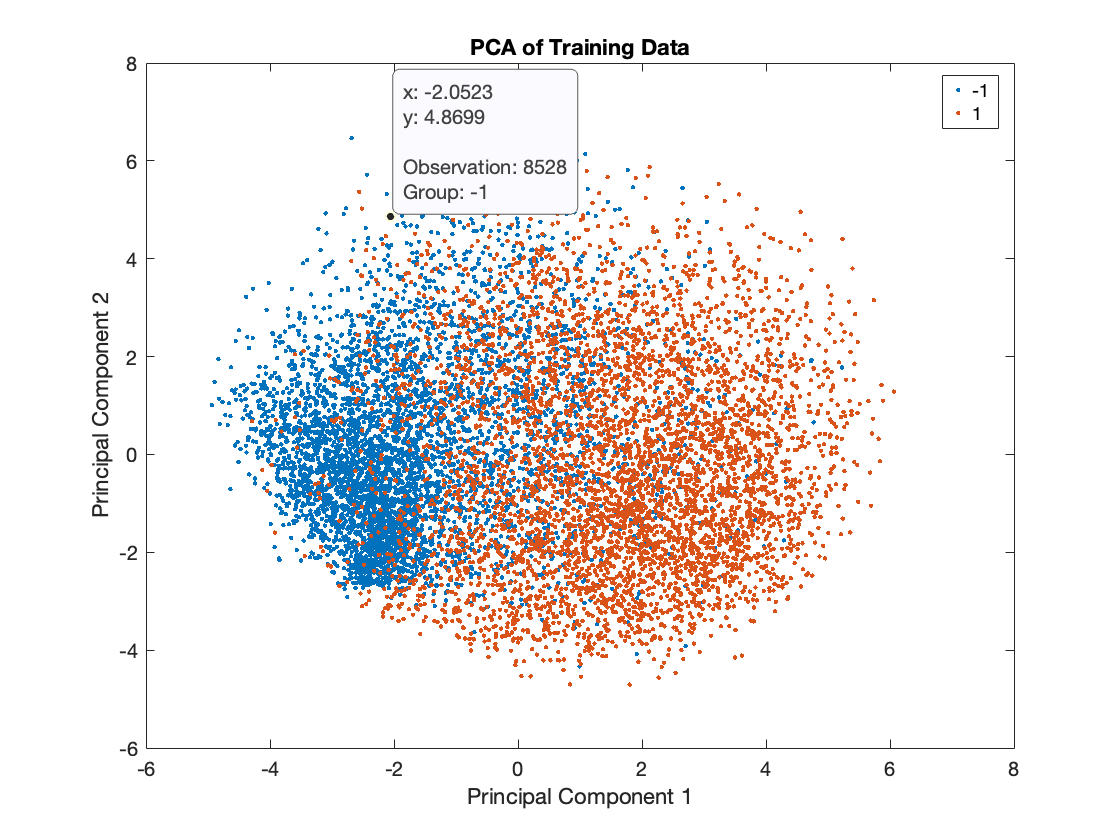
\includegraphics[width=\textwidth]{images/train_data.png}
    \caption{Training data distribution.}
    \label{fig:train_data}
  \end{subfigure}
  \begin{subfigure}[b]{0.45\textwidth}
    \centering
    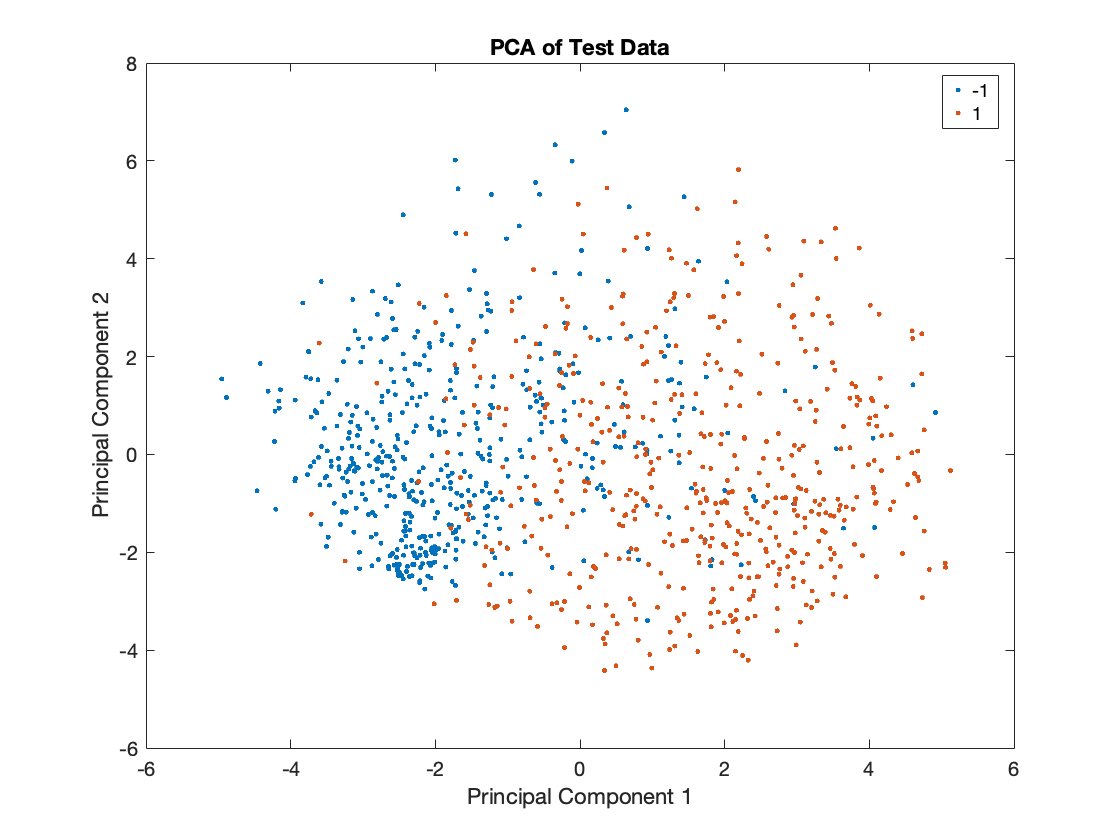
\includegraphics[width=\textwidth]{images/test_data.png}
    \caption{Test data distribution.}
    \label{fig:test_data}
  \end{subfigure}
  \caption{PCA projection of the training and test data}
  \label{fig:side_by_side_images}
\end{figure}
\subsubsection{a. Gradient Descent}
\begin{figure}[H]
  \centering
  \begin{subfigure}[b]{0.3\textwidth}
    \centering
    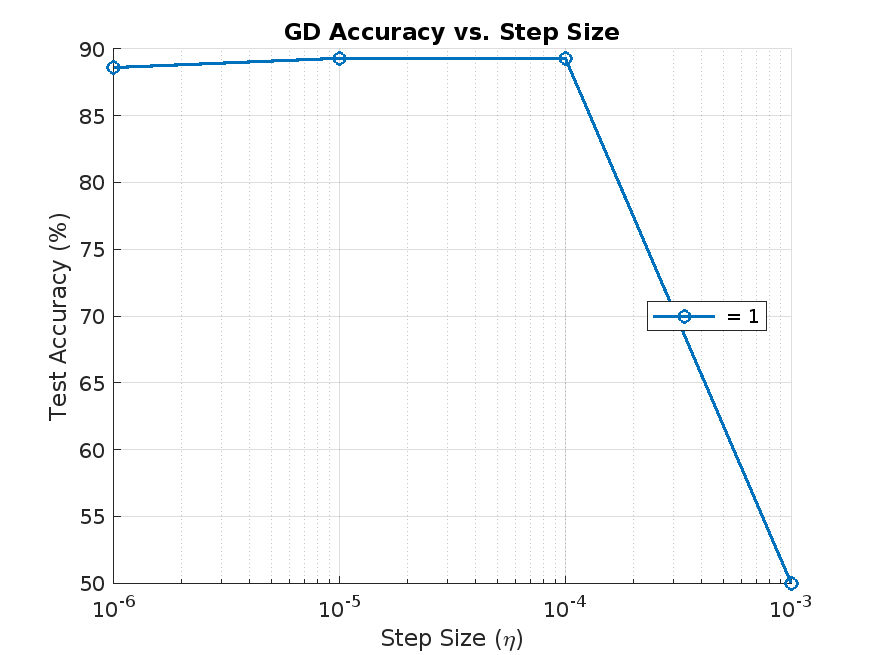
\includegraphics[width=\textwidth]{images/gd_accuracy_vs_step_size.png}
    \caption{Test accuracy vs step size}
    \label{fig:step_size_acc_gd}
  \end{subfigure}
  \begin{subfigure}[b]{0.3\textwidth}
    \centering
    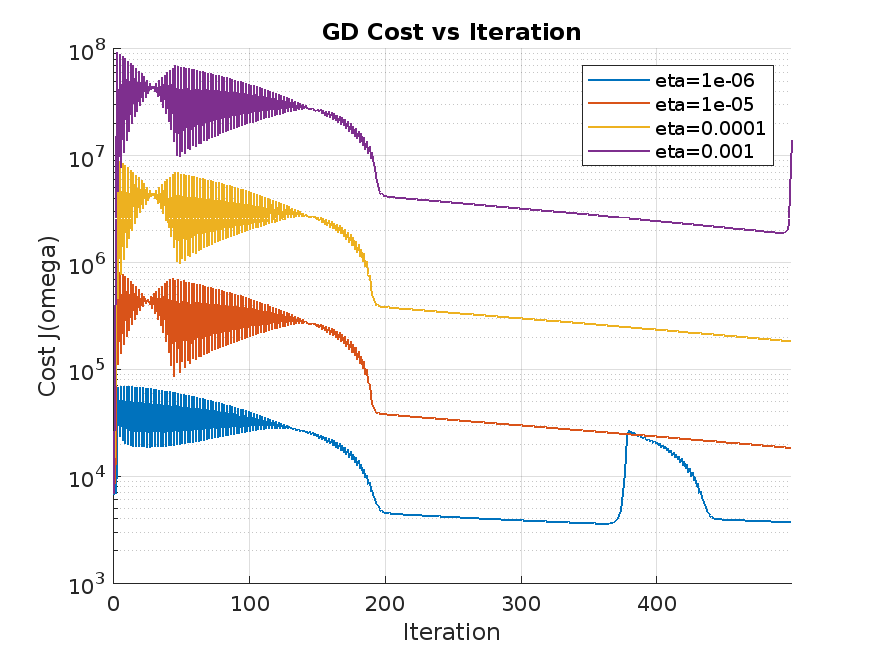
\includegraphics[width=\textwidth]{images/gd_cost_vs_iteration.png}
    \caption{Cost vs iteration}
    \label{fig:gd_cost}
  \end{subfigure}
  \begin{subfigure}[b]{0.3\textwidth}
    \centering
    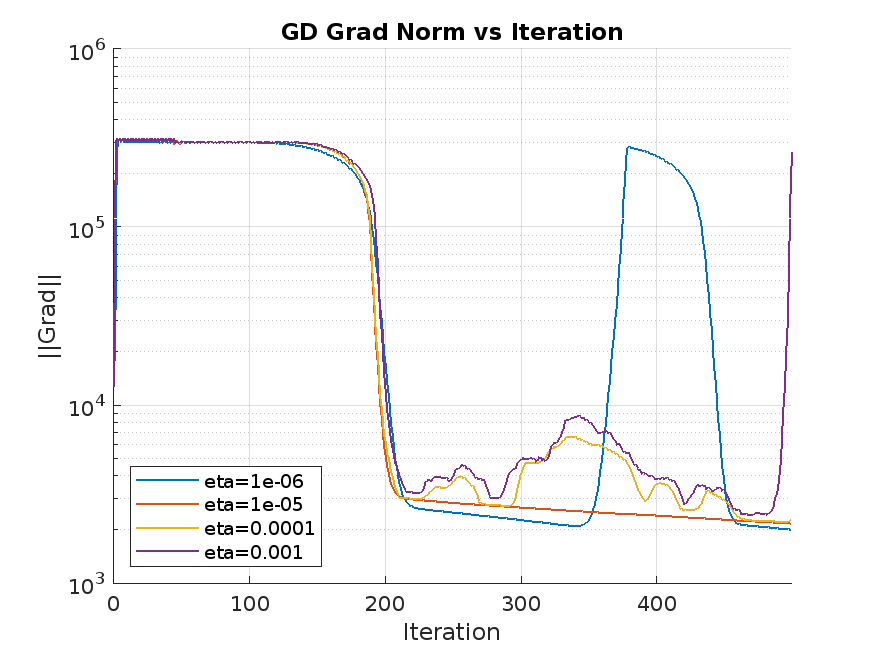
\includegraphics[width=\textwidth]{images/gd_grad_norm_vs_iteration.png}
    \caption{Gradient norm vs iteration}
    \label{fig:gd_grad_norm}
  \end{subfigure}
  \caption{Gradient Descent results}
  \label{fig:gd_results}
\end{figure}

\subsubsection{b. Stochastic Gradient Descent}

\begin{figure}[H]
  \centering
  \begin{subfigure}[b]{0.3\textwidth}
    \centering
    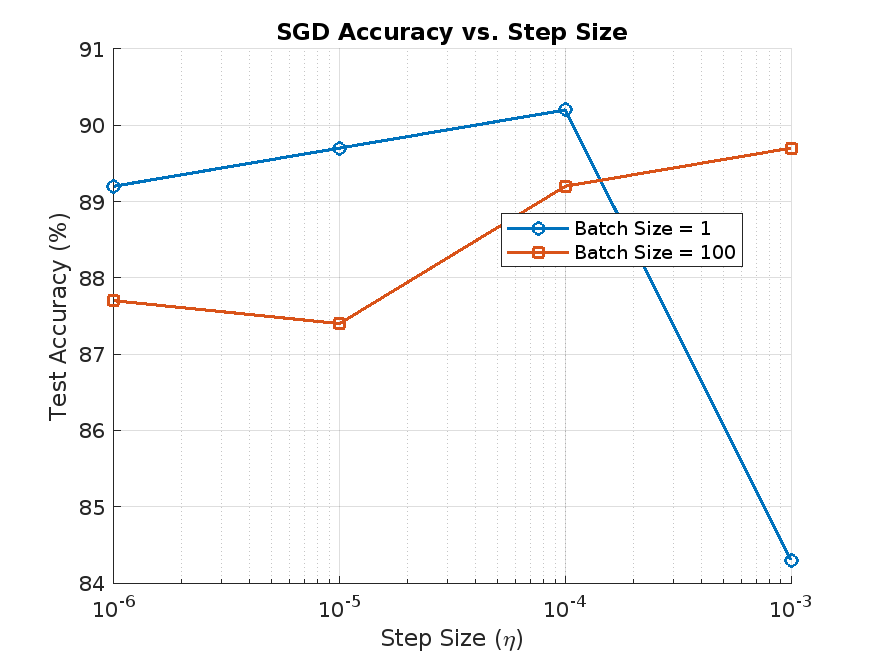
\includegraphics[width=\textwidth]{images/sgd_accuracy_vs_step_size.png}
    \caption{Test accuracy vs step size}
    \label{fig:step_size_acc_sgd}
  \end{subfigure}
  \begin{subfigure}[b]{0.3\textwidth}
    \centering
    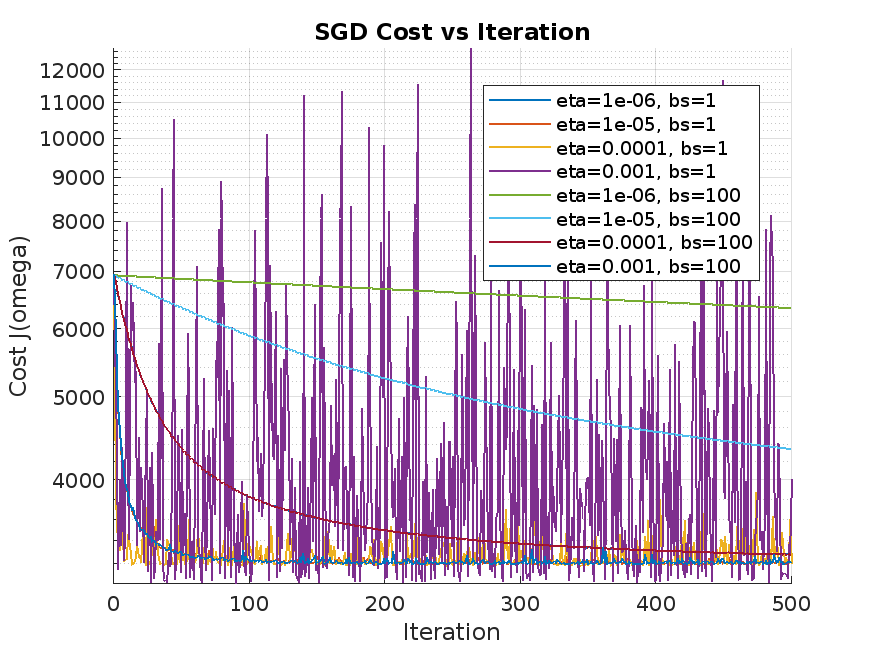
\includegraphics[width=\textwidth]{images/sgd_cost_vs_iteration.png}
    \caption{Cost vs iteration}
    \label{fig:sgd_cost}
  \end{subfigure}
  \begin{subfigure}[b]{0.3\textwidth}
    \centering
    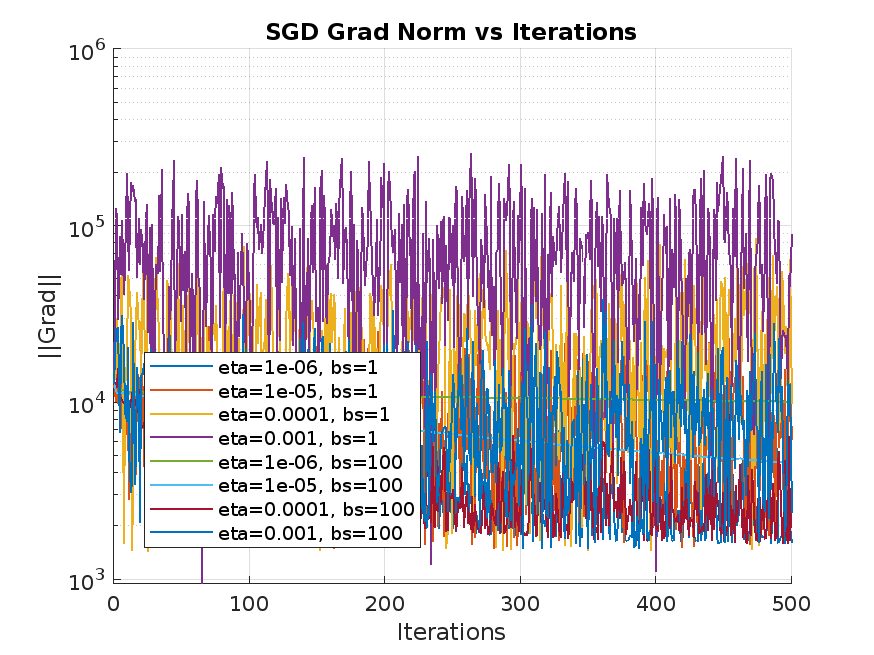
\includegraphics[width=\textwidth]{images/sgd_grad_norm_vs_iterations.png}
    \caption{Gradient norm vs iteration}
    \label{fig:sgd_grad_norm}
  \end{subfigure}
  \caption{Stochastic Gradient Descent results.}
  \label{fig:sgd_results}
\end{figure}

\subsubsection{c. BFGS}
\begin{figure}[H]
  \centering
  \begin{subfigure}[b]{0.45\textwidth}
    \centering
    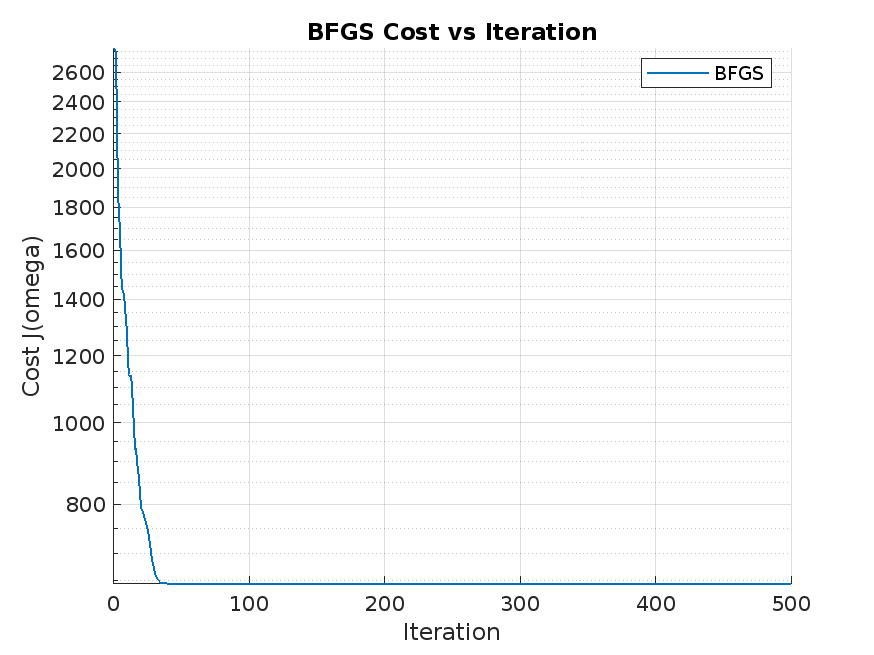
\includegraphics[width=\textwidth]{images/bfgs_cost_vs_iteration.png}
    \caption{Cost vs iteration}
    \label{fig:bfgs_cost}
  \end{subfigure}
  \begin{subfigure}[b]{0.45\textwidth}
    \centering
    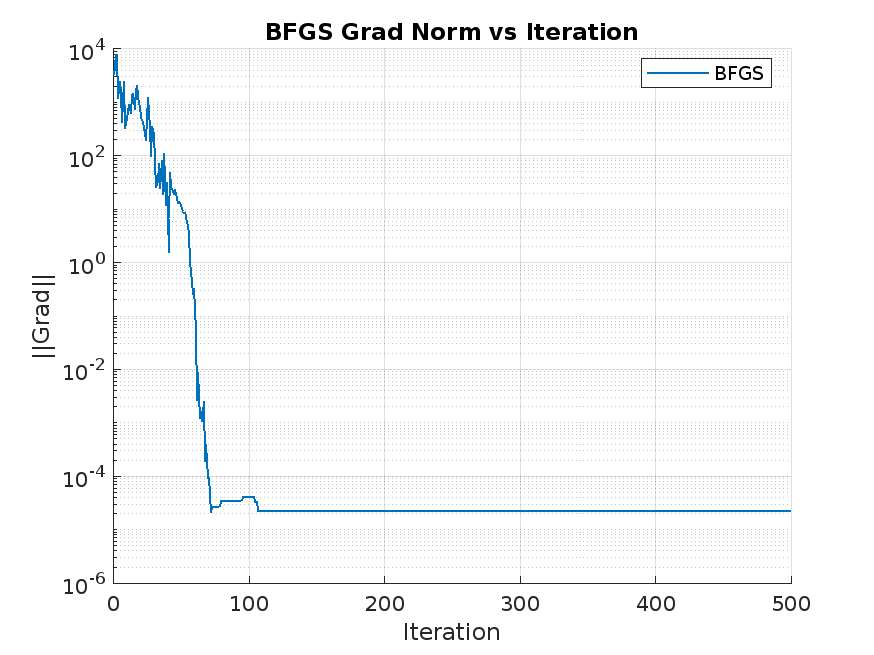
\includegraphics[width=\textwidth]{images/bfgs_grad_norm_vs_iteration.png}
    \caption{Gradient norm vs iteration}
    \label{fig:bfgs_grad_norm}
  \end{subfigure}
  \caption{BFGS results}
  \label{fig:bfgs_results}
\end{figure}
\subsubsection{d. L-BFGS}

\begin{figure}[H]
  \centering
  \begin{subfigure}[b]{0.3\textwidth}
    \centering
    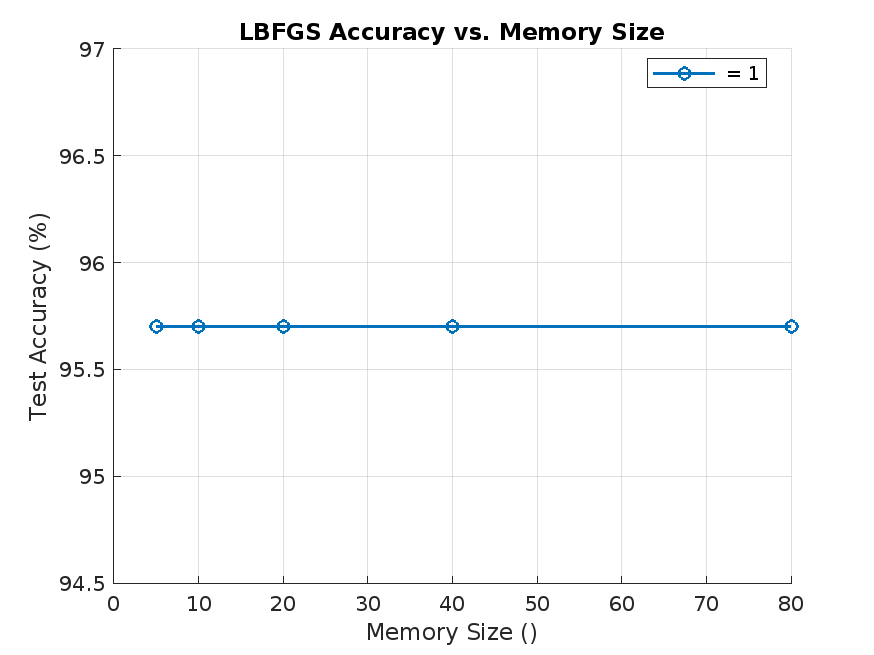
\includegraphics[width=\textwidth]{images/lbfgs_accuracy_vs_memory_size.png}
    \caption{Test accuracy vs memory size}
    \label{fig:step_size_acc_lbfgs}
  \end{subfigure}
  \begin{subfigure}[b]{0.3\textwidth}
    \centering
    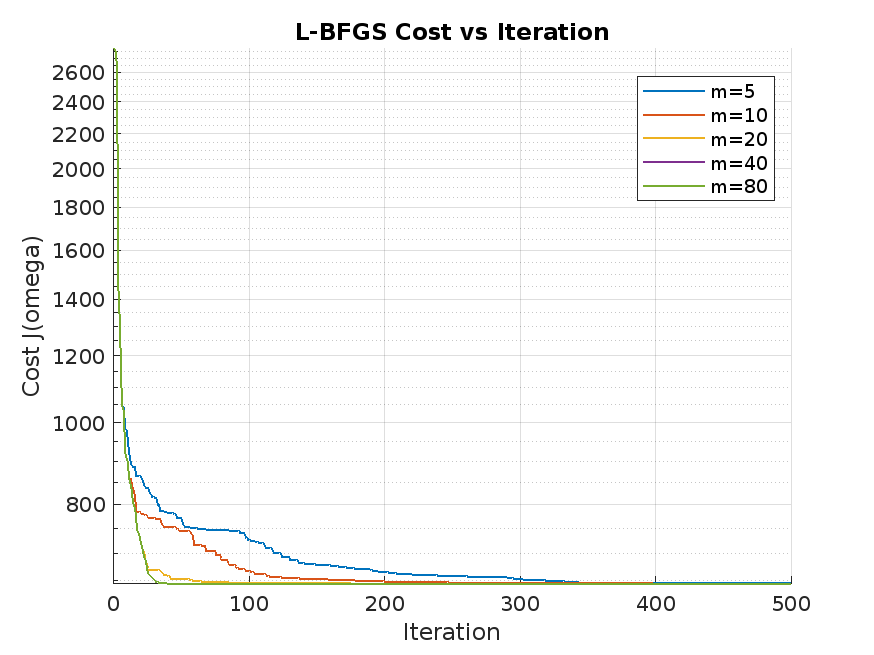
\includegraphics[width=\textwidth]{images/lbfgs_cost_vs_iteration.png}
    \caption{Cost vs iteration}
    \label{fig:lbfgs_cost}
  \end{subfigure}
  \begin{subfigure}[b]{0.3\textwidth}
    \centering
    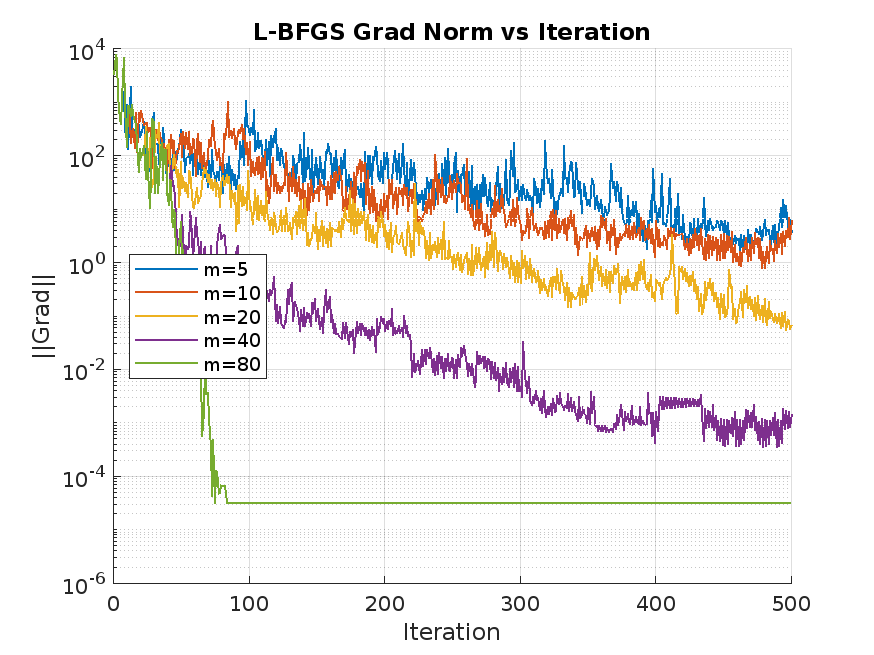
\includegraphics[width=\textwidth]{images/lbfgs_grad_norm_vs_iteration.png}
    \caption{Gradient norm vs iteration}
    \label{fig:lbfgs_grad_norm}
  \end{subfigure}
  \caption{Stochastic Gradient Descent results.}
  \label{fig:lbfgs_results}
\end{figure}

\subsubsection{Analysis of Results}
Table~\ref{tab:summary_results} summarizes the performance of each optimizer on the kernel logistic regression task. The table lists the best parameters (if any), test accuracy, number of iterations (or epochs), the final gradient norm, and the final cost.
\begin{table}[H]
  \centering
  \begin{tabular}{@{}llcccc@{}}
    \toprule
    \textbf{Optimizer} & \textbf{Parameters} & \textbf{Test Acc. (\%)} & \textbf{Iterations} & \textbf{$\|\nabla J(\omega)\|$} & \textbf{$J(\omega)$} \\ \midrule
    GD     & $\eta = 1\times10^{-5}$             & 89.30 & 500  & 2171      & 18542.3 \\ 
    SGD    & $\eta = 1\times10^{-4},\, bs=1$      & 90.20 & 500  & 9742.64   & 3190.68 \\ 
    BFGS   & ---                               & 95.70 & 500  & $2.30\times10^{-5}$ & 645.275 \\ 
    L-BFGS & $m = 5$                          & 95.70 & 500  & 3.53      & 645.487 \\ \bottomrule
  \end{tabular}
  \caption{Summary of optimizer parameters and final performance results.}
  \label{tab:summary_results}
\end{table}
\noindent Figure~\ref{fig:best_runs} illustrates a visual comparison among the best runs of the optimizers. Figure~\ref{fig:pca_best_runs} (left) shows the PCA projections of the predictions, while Figure~\ref{fig:convergence_best_runs} (right) displays the cost versus iterations.
\begin{figure}[H]
  \centering
  \begin{subfigure}[b]{0.45\textwidth}
    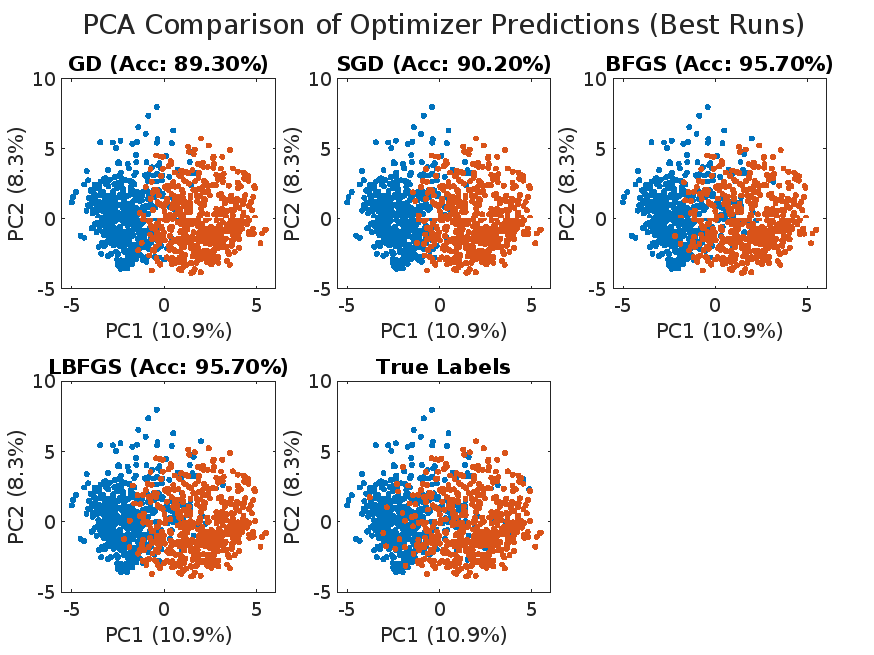
\includegraphics[width=\textwidth]{images/pca_predictions_comparison_Best_Runs.png}
    \caption{PCA Projection of Predictions}
    \label{fig:pca_best_runs}
  \end{subfigure}
  \begin{subfigure}[b]{0.45\textwidth}
    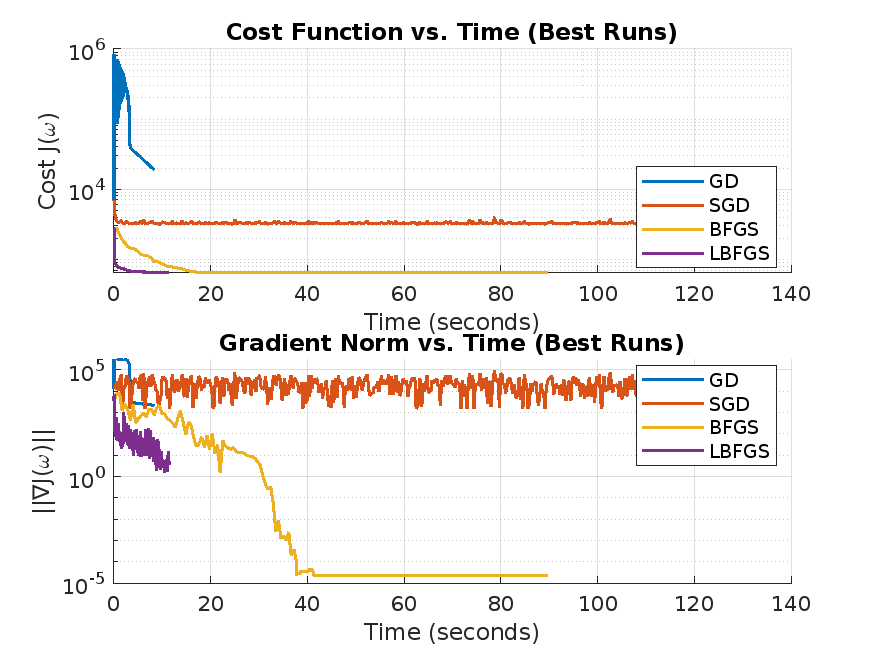
\includegraphics[width=\textwidth]{images/convergence_comparison_Best_Runs.png}
    \caption{Cost vs. Iterations}
    \label{fig:convergence_best_runs}
  \end{subfigure}
  \caption{Comparison of the best runs across all optimizers.}
  \label{fig:best_runs}
\end{figure}
\paragraph{Log Summary:}
The detailed logs include iteration-by-iteration metrics such as cost, gradient norm, step sizes, and curvature condition warnings. These logs offer additional insights into the behavior of the optimizers and can serve as a diagnostic tool for further tuning. The summary of the logs is as follows:
\begin{itemize}
  \item GD and SGD failed to meet the gradient tolerance within 500 iterations/epochs, resulting in consistently larger gradient norms.
  \item BFGS shows rapid cost reduction and very low gradient norms, but the logs include numerous warnings about curvature conditions not being met, resulting in skipped Hessian updates.
  \item L-BFGS with various memory sizes also attains low cost values and high accuracy, although the gradient norm is higher than in BFGS, possibly due to less complete convergence under the limited-memory approximation.
\end{itemize}
\paragraph{Key Observations:}
\begin{itemize}
  \item \textbf{Quasi-Newton Methods Lead:} Both BFGS and L-BFGS attain a test accuracy of 95.70\% despite operating on a reduced training set (4000 samples), outperforming the full-dataset first-order methods (GD and SGD) which reach roughly 89--90\%.
  \item \textbf{Convergence Quality:} BFGS achieves a very low final gradient norm ($\sim2.30\times10^{-5}$), indicating strong convergence. In contrast, L-BFGS, while reaching a similar final cost, ends with a higher gradient norm (approximately 3.53), suggesting that it did not converge as completely within 500 iterations. Nevertheless, this does not affect its test accuracy.
  \item \textbf{GD and SGD Sensitivity:} GD is highly sensitive to the choice of learning rate, with the best performance observed at $\eta = 1\times10^{-5}$. SGD, though slightly less sensitive, still requires careful tuning to achieve its best result.
  \item \textbf{Memory Parameter in L-BFGS:} Experiments with different memory sizes (from $m=5$ up to $m=80$) yield similar final accuracy, indicating that a small memory (e.g., $m=5$) is sufficient to capture the necessary curvature information for this task.
\end{itemize}

\paragraph{Conclusion:}
For this kernel logistic regression problem, quasi-Newton methods (BFGS and L-BFGS) outperform first-order methods (GD and SGD) in both accuracy and convergence speed. Even when using a significantly reduced training set, these second-order methods achieve substantially higher accuracy and lower final cost. The strong performance of L-BFGS, even with a small memory size, demonstrates its effectiveness as a computationally efficient alternative to full BFGS for large-scale problems.

\medskip


\section{Code}
\subsection{Dataset Code}
\lstinputlisting[language=Matlab]{../code/data.m}
\subsection{Experiment Code}
\lstinputlisting[language=Matlab]{../code/main.m}
\subsection{Optimizer Code}
\subsubsection{Gradient Descent}
\lstinputlisting[language=Matlab]{../code/gd_optimizer.m}
\subsubsection{Stochastic Gradient Descent}
\lstinputlisting[language=Matlab]{../code/sgd_optimizer.m}
\subsubsection{BFGS}
\lstinputlisting[language=Matlab]{../code/bfgs_optimizer.m}
\subsubsection{L-BFGS}
\lstinputlisting[language=Matlab]{../code/lbfgs_optimizer.m}
\subsection{Evaluation Code}
\lstinputlisting[language=Matlab]{../code/evaluate_model.m}
\lstinputlisting[language=Matlab]{../code/kernelLogisticCostGrad.m}
\subsection{Plotting Code}
\subsubsection{Plot Convergence}
\lstinputlisting[language=Matlab]{../code/plot_convergence.m}
\subsubsection{Plot Cost vs Iteration}
\lstinputlisting[language=Matlab]{../code/plot_iteration_convergence.m}
\subsubsection{Plot Accuracy vs Hyperparameters}
\lstinputlisting[language=Matlab]{../code/plot_accuracy_hyperparam.m}
\subsubsection{Plot PCA Predictions}
\lstinputlisting[language=Matlab]{../code/plot_pca_predictions.m}

\section{References}

\begin{enumerate}
    \item Bishop, C. M. (2006). Pattern Recognition and Machine Learning. Springer.
    \item Advanced Machine Learning Lecture Notes 6
    \item \href{https://www.youtube.com/watch?v=QGFct_3HMzkURL}{Quasi Newton and BFGS}
    \item \href{https://www.youtube.com/watch?v=VIoWzHlz7k8}{Understanding scipy.minimize part 1: The BFGS algorithm}
    \item \href{https://www.youtube.com/watch?v=kM79eCS9cs8}{Understanding scipy.minimize part 2: Line search}
\end{enumerate}

\end{document}
